\subsection{Advanced Plotting - Palm - Chapter 5}

\begin{enumerate}

\item {\bf 2-Dimensional Plots}

Here we will focus on plotting. We already know how to evaluate
functions using the dot operator. For example, the code below will
evaluate the trajectory of a projectile launched at 45 degrees.

\begin{framed}

theta = pi/4;

V = 10;

vy = V*sin(theta); vx = V*cos(theta);

timestep = 0.1;

t = 0:timestep:3;

x0 = 0; y0 = 0;

x = x0 + vx*t;

g = 9.81;

y = y0 + vy*t - (1/2)*g*t.\textrm{\^}2;

\end{framed}

To plot this function we merely use the plot command. 

$>>$ plot(x,y)

Running this command from the command window will open a default plot
with a blue line. However, the plot will be pretty mundane. The code
below will make the figure look alot better.

\begin{framed}

\textcolor{OliveGreen}{\% Close all other figures then, create a figure and name it Trajectory}

close all 

fig = figure('Name','Trajectory'); 

\textcolor{OliveGreen}{\% Set the background of the figure to white.}

set(fig,'color','white') 

\textcolor{OliveGreen}{\% Change the fontsize of the figure to 18}

set(axes,'FontSize',18) 

\textcolor{OliveGreen}{\% Plot x and y with a red dashed line with a line width of 2}

plot(x,y,'r--','LineWidth',2) 

\textcolor{OliveGreen}{\% Turn on the grid}

grid on 

\textcolor{OliveGreen}{\% Label the axes and make the font size 18}

xlabel('X (m)')

ylabel('Y (m)')

title('Trajectory of a Ball');

\end{framed}

Running the code above produces the figure below. 

\begin{figure}[htb]
  \begin{center}
    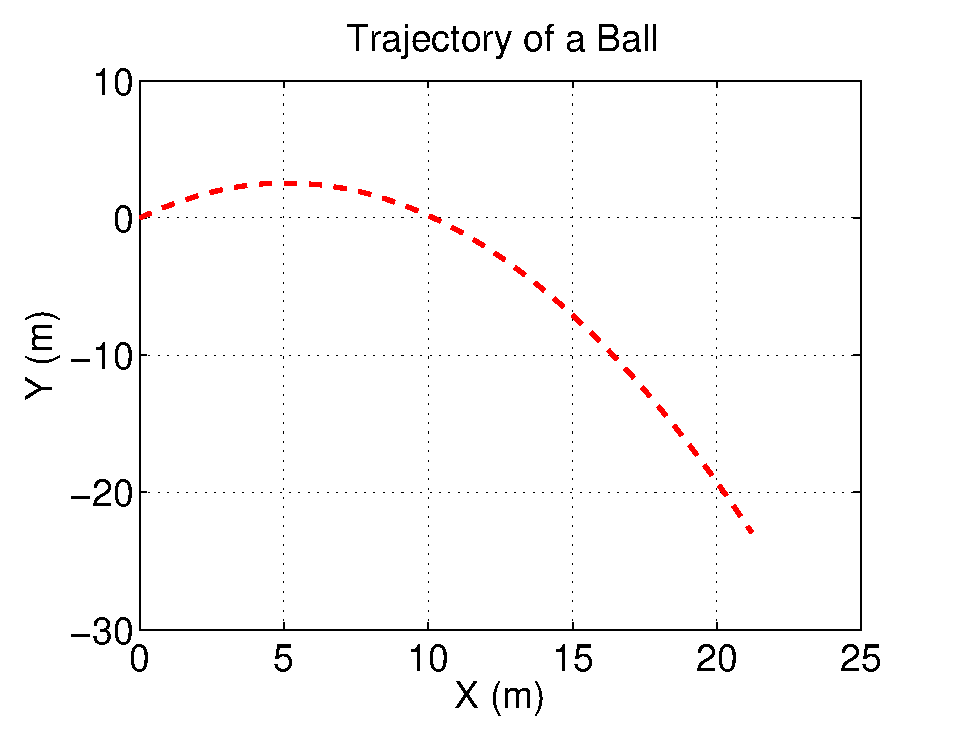
\includegraphics[height=0.45\textwidth,width=0.6\textwidth]{Graphics/Example_Plot}
  \end{center}
\end{figure}

Notice, that the projectile falls through the ground. It is beneficial
to restrict the axis so as to only see the plot when the ball hits the
ground. Extra code must be added to find when the ball hits the
ground. The code below computes when the ball hits the ground and then
restricts the axis to this window. In addition, the maximum height is
computed.

\begin{framed}

tground = 2*vy/g;

tmax\_height = tground/2;

xground = x0 + vx*tground;

ymax = y0 + vy*tmax\_height - (1/2)*g*tmax\_height\textrm{\^}2;

axis([0 xground 0 ymax])

\end{framed}

The result of the code above creates the figure below. 

\begin{figure}[htb]
  \begin{center}
    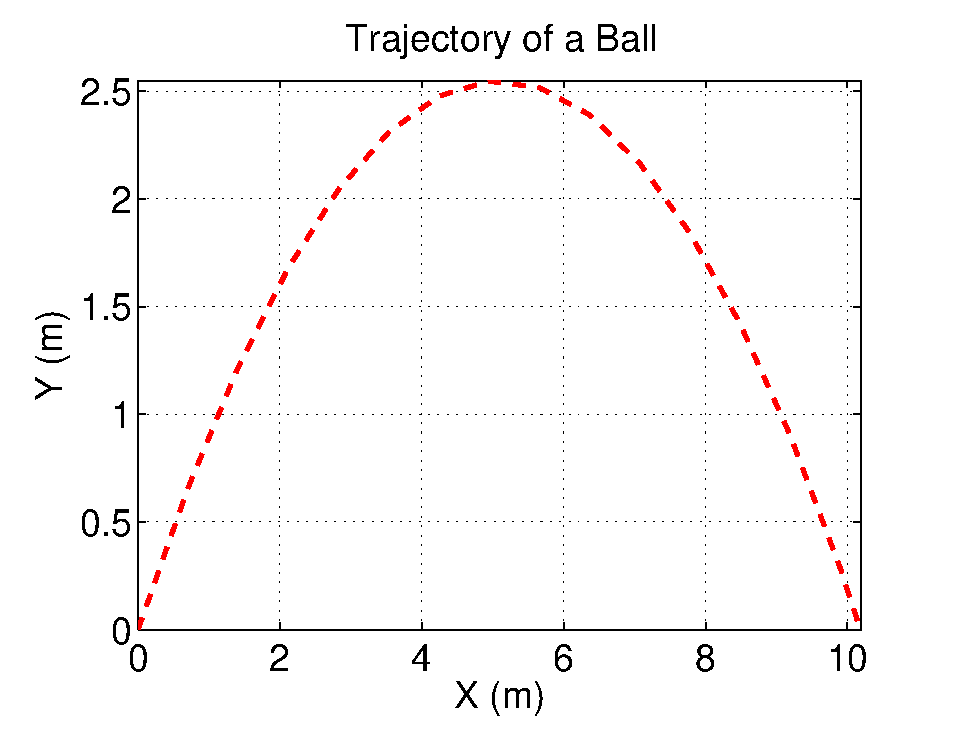
\includegraphics[height=0.45\textwidth,width=0.6\textwidth]{Graphics/Example_Plot_Small}
  \end{center}
\end{figure}

\item {\bf 3-D Plotting} 

MATLAB can also plot in three dimension. Let's assume for example we
wish to plot a helical pattern. The equation of a helix can be done by
creating a linear equation for the z-coordinate and a circular pattern
for the x and y coordinates.

\begin{framed}

theta = 0:0.01:(6*pi);

x = cos(theta);

y = sin(theta);

z = linspace(-1,1,length(theta));

plot3(x,y,z)

\end{framed}

After including grids, and labels the figure below is created. 

\begin{figure}[htb]
  \begin{center}
    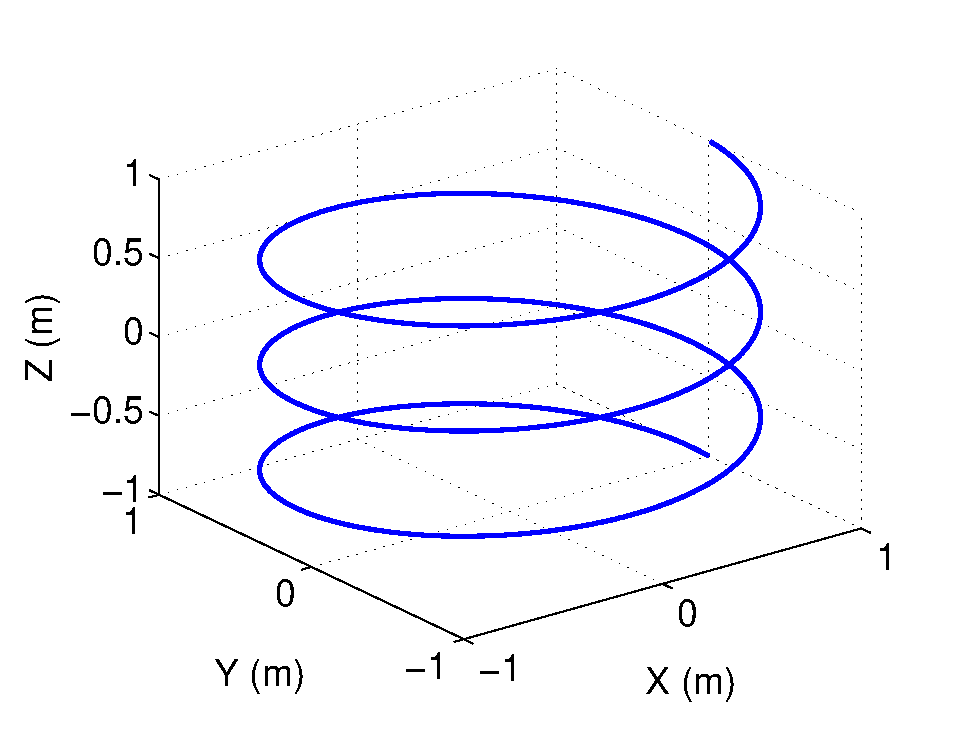
\includegraphics[height=0.55\textwidth,width=0.7\textwidth]{Graphics/Helical}
  \end{center}
\end{figure}

\item {\bf Meshing}

Meshing can be used to plot 3D surfaces as well as 3D solids. The code
below creates a 3D surface and then meshes the figure shown below. The
line meshgrid is used to create an array from the 1-D x and y vectors.

\begin{framed}

x = linspace(-5,5,100);

y = linspace(-5,5,100);

[xx,yy] = meshgrid(x,y);

zz = xx.\textrm{\^}2 + yy.\textrm{\^}2;

mesh(xx,yy,zz);

\end{framed}

Note again, that extra code was added to create a grid and labels,
etc. 

\clearpage

\begin{figure}[htb]
  \begin{center}
    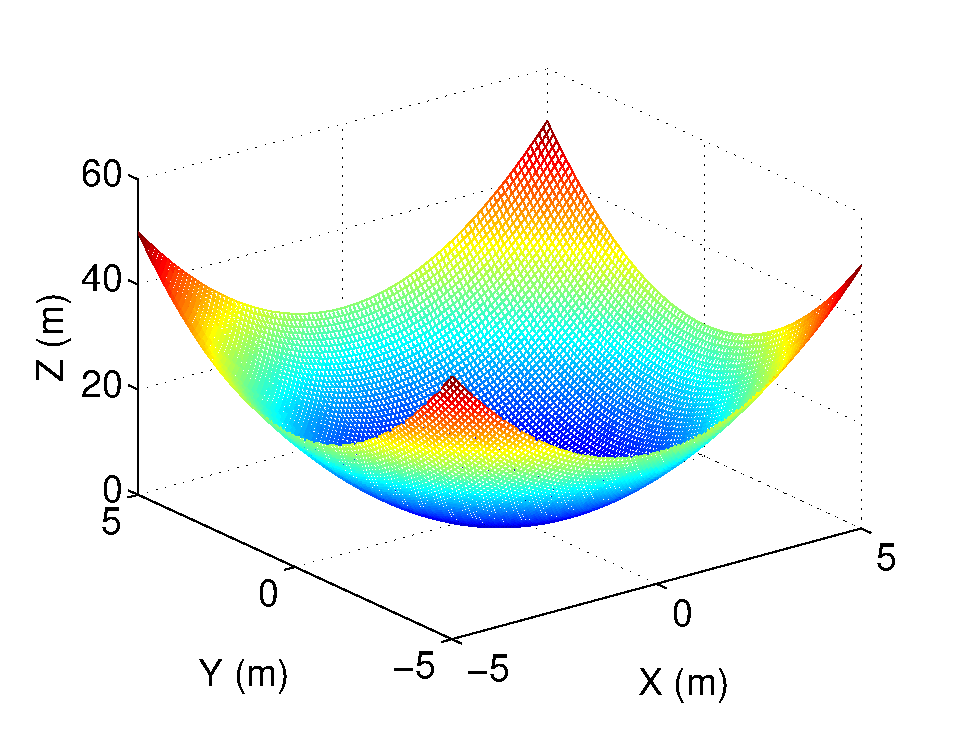
\includegraphics[height=0.55\textwidth,width=0.7\textwidth]{Graphics/Meshing}
  \end{center}
\end{figure}

It is also possible to create 3-D solids using a stacking
algorithm. That is, it is possible to stack 2-D objects on top of each
other. The code below plots a 2-D square in 3-dimensions. 

\begin{framed}

x = [-1 1 1 -1 -1];

y = [-1 -1 1 1 -1];

z = [0 0 0 0 0];

plot3(x,y,z);

\end{framed}

Stacking more squares on top of each other you can create a
rectangular prism. However, if you stack smaller and smaller squares
it is possible to make a pyramid. The code below creates a pyramid
using a stacking algorithm. Note that the [~] brackets are used to
create empty vectors. The last line of code is used to orient the
camera to view the pyramid at an elevation of 30 degrees and an
azimuth of -27. 

\begin{framed}

radius = 1;

xx = [~];yy = [~];zz = [~];

while radius $>=$ 0

~~~~~~~~xx = [xx;radius*x];

~~~~~~~~yy = [yy;radius*y];

~~~~~~~~zz = [zz;z];

~~~~~~~~z = z + 1;

~~~~~~~~radius = radius - 0.1;

end

mesh(xx,yy,zz)

view(-27,30)

\end{framed}

\begin{figure}[htb]
  \begin{center}
    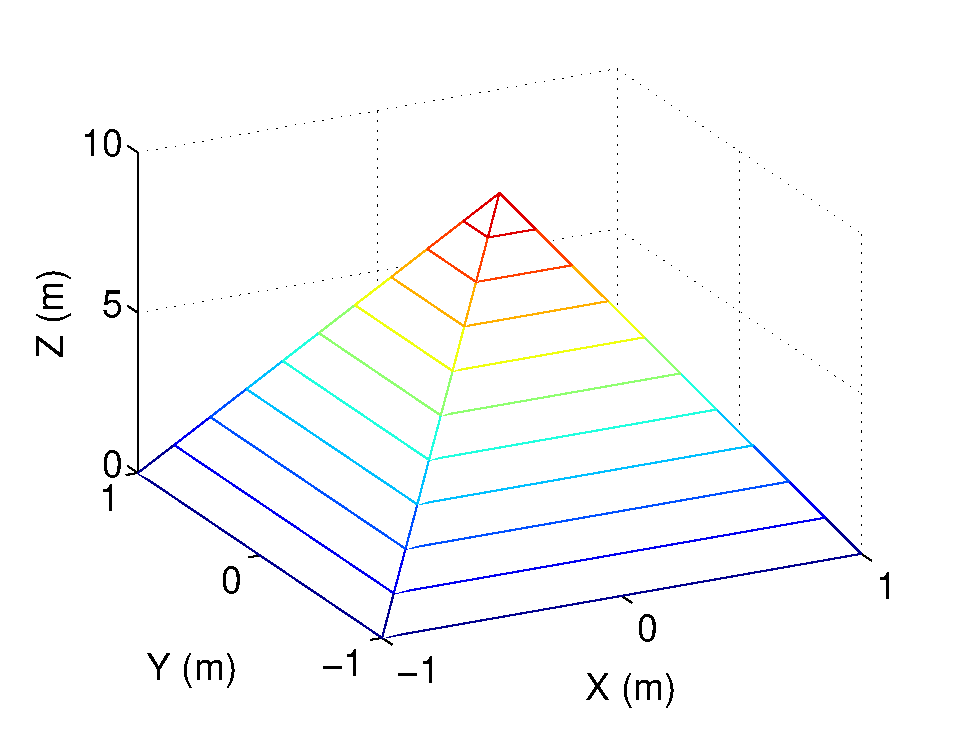
\includegraphics[height=0.55\textwidth,width=0.7\textwidth]{Graphics/Pyramid}
  \end{center}
\end{figure}

\item {\bf Animating }

Animating is actually very simple. The code below animates the ball
flying through the air assuming you have the x and y values defined
from above.

\begin{framed}

for idx = 1:length(x)

~~~~~~~cla;

~~~~~~~plot(x(1:idx),y(1:idx),'b-','LineWidth',2)

~~~~~~~hold on

~~~~~~~plot(x(idx),y(idx),'bs','MarkerSize',10)

~~~~~~~axis([0 xground 0 ymax])

~~~~~~~drawnow

end

\end{framed}

The way this code works is by intelligently using cla and drawnow. cla
clears the current figure. The lines inbetween cla and drawnow serve
to plot the ball at the current position in the loop. Drawnow is then
used to create a frame such that you and I can see it in real
time. That is, every loop in the for loop creates a frame. A movie is
really just a sequence of frames plotted one after the other. 

\end{enumerate}
